\documentclass{article}
\usepackage[utf8]{inputenc}
\usepackage{graphicx}
\graphicspath{{./images/}}
\usepackage{subfig}
\usepackage{caption}

%\title{Algebra Linear - PCA}
%\author{Josiel Santana}
%\date{December 2022}

\begin{document}
\thispagestyle{empty}

\begin{center}
    
\includegraphics[width=8cm]{fateclogo.png}\\
    \vspace{1cm}
    \textbf{Fatec Baixada Santista - Rubens Lara}\\
    Ciência de Dados - 2° Ciclo\\
    \vspace{4.4cm}
    \textbf{Principal Component Analysis (PCA)}\\
    \textbf{Atividade - Álgebra Linear }\\
    \vspace{4.4cm}
    \textbf{Josiel Santana de Medeiros}\\
    \textbf{Stefany de Oliveira Fernandes}\\
    \vspace{4.4cm}
    \textbf{Santos - SP}\\
    \textbf{Dezembro/2022}
\end{center}

\clearpage
\setcounter{page}{1}

\section{Introdução}
\section*{Conceito de PCA}
\begin{flushleft}
    A Análise de Componentes Principais, ou Principal Component Analysis (PCA), consiste em uma técnica que transforma dados com várias dimensões em dimensões menores, tentando manter o máximo de informação possivel.
    \newline
    Essa técnica é útil em vários casos, principalmente em que há um dataset com várias features, como, por exemplo, em processamento de imagens ou pesquisa de genomas.
\end{flushleft}

\section*{Escolha do Dataset}
\begin{flushleft}
    Para fazer esse trabalho, foi escolhido um dataset da Copa do Mundo da Fifa disponibilizado no Kaggle, que contém dados das edições de 1930 até 2014. Nele haviam três tabelas, sendo elas: todos os jogadores que já participaram de alguma edição, todas as partidas e todos os vencedores do evento. Nesse trabalho será usada apenas a tabela com os vencedores da Copa do Mundo, que nesse caso é o arquivo \emph{WorldCups.csv}.
    \begin{figure}[h]
        \centering
        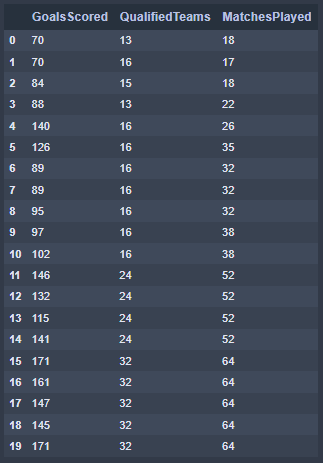
\includegraphics[scale=0.6]{tabelatratada}
        \caption{Dataset utilizado para o trabalho.}
        \label{fig:x cubed graph}
    \end{figure}
\end{flushleft}

\newpage
\section{Processo}
\section*{Tratamento do Dataset}
\begin{flushleft}
    Usando da biblioteca \textbf{Pandas}, o dataset foi importado e foram definidos as colunas que serão \textbf{inputs e outputs}. Selecionamos as colunas de 'GoalsScored', 'QualifiedTeams' e 'MatchesPlayed' para serem as três variáveis de inputs (X) e o nome das classes dos vencedores para como output (Y), essa que contém 20 países: 'Uruguay', 'Italy', 'Argetina', 'France', entre outros.
    \newline
    Outras colunas que estavam nesse dataset e continham nomes, como 'Country' ou 'Runners' foram desprezadas, pois a análise se aplica apenas para analisar dados quantitativos.
    \newline
    Com isso, temos os inputs com a dimensão de 20 linhas e 3 colunas (20,3) e os outputs com dimensão de 20 linhas (20,).
\end{flushleft}

\section*{Definido o número de Principal Components}
\begin{flushleft}
    Nessa etapa foram usados dois módulos da biblioteca \textbf{Sklearn}, no caso a \textbf{Preprocessing} e a \textbf{Decomposition}. Com isso, já pode ser usada a função PCA do módulo Decomposition, onde foi definido como \textbf{dois} a quantidade de Principal Components. 
    \newline
    Vale considerar que o número de componentes principais é sempre menor ou igual ao número de variáveis originais, então também seria possível definir o número de componentes como 3.
\end{flushleft}

\section*{Valores de Scores}
\begin{flushleft}
    Tendo essas colunas, era necessário fazer uma transformação nesses dados para todos terem o mesmo peso, para isso foi calculado o scores dessas variáveis:
\end{flushleft}
\begin{figure}[h!]
    \centering
    \subfloat{{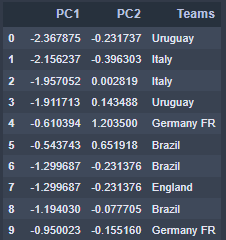
\includegraphics[width=4.7cm]{scores1} }}%
    \qquad
    \subfloat{{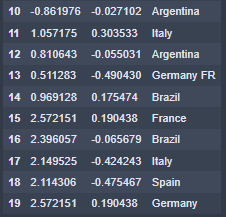
\includegraphics[width=5.2cm]{scores2} }}%
    \label{fig:example}%
    \caption{Dataset após o cálculo dos scores junto com a coluna de vencedores.}
\end{figure}

\section*{Valores de Loadings}
\begin{flushleft}
    Após ter os scores foi feito também uma tabela com os valores de loading, sendo uma linha para cada um dos 3 descritores, ou seja, 'GoalsScored', 'QualifiedTeams' e 'MatchesPlayed'
\end{flushleft}

\section*{Variância Explicada}
\begin{flushleft}
    Para explicar a contribuição de cada um dos 2 componentes principais na variância do dataset foi feito o calculo da variância explicada. Os resultados para o primeiro e segundo componente foram de aproximadamente 93\% e 5\%.
\end{flushleft}

\section*{Variância Cumulativa}
\begin{flushleft}
    Com os valores dos dois componentes, 93\% e 5\%, foi feita uma soma cumulativa, resultando numa matriz de aproximadamente 93\% e 98\%. Com isso é possível concluir que o \textbf{PC1 e o PC2 representam cerca de 98\% da variância}.
\end{flushleft}

\newpage

\section{Visualização}
\begin{flushleft}
    Nessa etapa foram usadas as bibliotecas \textbf{Numpy}, para manipular as matrizes e para usar as funções matemáticas, e o \textbf{Plotly Express}, com o objetivo de plotar os gráficos.
\end{flushleft}

\section*{Variância Explicada e Cumulativa}
\begin{flushleft}
    Foi feito uma junção de dois gráficos, o gráfico de barras (trace 1) representa a variância explicada dos dois componentes e o gráfico de linha (trace 2) representa a variância acumulada.
\end{flushleft}
\begin{figure}[h]
    \centering
    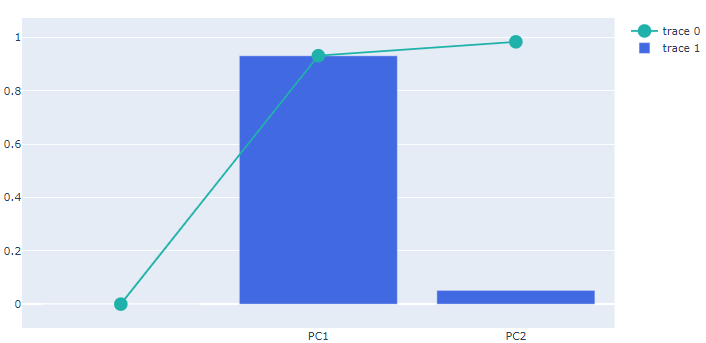
\includegraphics[scale=0.4]{varianciaexplicada}
    \caption{Multi plot graph com a variância explicada e cumulativa em decimal.}
    \label{fig:x cubed graph}
\end{figure}

\section*{Mapa de Calor}
\begin{flushleft}
    Também foi feito um gráfico do tipo Heatmap para entender quanto os componentes principais representam em cada coluna.
\end{flushleft}
\begin{figure}[h]
    \centering
    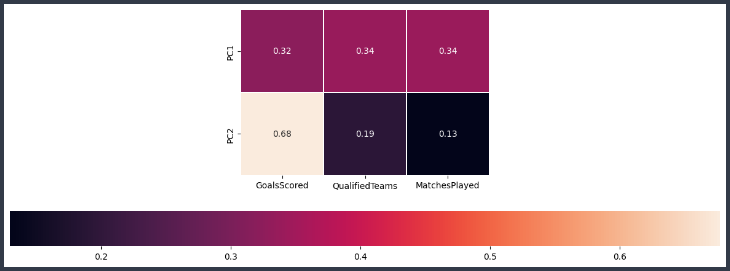
\includegraphics[scale=0.37]{mapadecalor}
    \caption{Heatmap dos componentes principais.}
    \label{fig:x cubed graph}
\end{figure}
\begin{flushleft}
    É possível concluir que o PC1 consiste em 32\% da coluna GoalsScored e 34\% das colunas QualifiedTeams e MatchesPlayed. O PC2 é composto por 68\% dos GoalsScored, 19\% dos QualifiedTeams e 13\% dos MatchesPlayed.
\end{flushleft}

\section*{Dados com os Componentes Principais}
\begin{flushleft}
    Por último, esses dados foram plotados em um gráfico de pontos, com o eixo X sendo o primeiro componente principal e o eixo Y sendo o segundo componente principal. Com isso, é demostrado como as dimensões desse dataset foram transformados, passando de três para apenas duas.
\end{flushleft}
\begin{figure}[h]
    \centering
    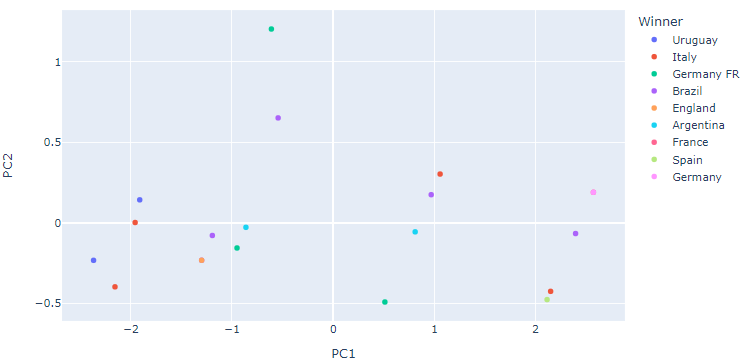
\includegraphics[scale=0.5]{pca}
    \caption{Gráfico final com os componentes principais após o tratamento com o PCA.}
    \label{fig:x cubed graph}
\end{figure}

\newpage
\section{Referências}
\begin{itemize}
  \item Data Professor - Machine Learning in Python: Principal Component Analysis (PCA) for Handling High-Dimensional Data: 
  \newline \emph{www.youtube.com/watch?v=oiusrJ0btwA}
  \item Casey Cheng - Principal Component Analysis (PCA) Explained Visually with Zero Math: 
  \newline \emph{towardsdatascience.com/principal-component-analysis-pca-explained-visually-with-zero-math-1cbf392b9e7d}
  \item Ecologia Descomplicada - Aula PCA simplificada: 
  \newline \emph{www.youtube.com/watch?v=KqZAC4jyJKc}
  \item Eduardo - Ciência dos Dados - ENTENDENDO DE VEZ O QUE É PCA - PRINCIPAL COMPONENT ANALYSIS: 
  \newline \emph{www.youtube.com/watch?v=p4bvCFygfW0}
  \item Gayathri Siva - PCA — Principal Component Analysis Explained with Python Example:
  \newline \emph{gayathri-siva.medium.com/pca-principal-component-analysis-explained-with-python-example-e403f9fef52b}
\end{itemize}

\vspace{4cm}
\begin{center} 
    \textbf{Repositório do Github:}
    https://github.com/StefanyFernandes675/PCA-worldCup \\
    \textbf{Dataset utilizado:}
    https://www.kaggle.com/datasets/abecklas/fifa-world-cup.
\end{center} 

\end{document}
